\documentclass[tikz]{standalone}
\usepackage{pgfplots}
\usepgfplotslibrary{groupplots}
\pgfplotsset{compat=1.18}
\begin{document}
% Generated by discussion_5_export_ac_parameter_tikz.py.
% Preamble: \usepackage{pgfplots}
%           \usepgfplotslibrary{groupplots}
%           \pgfplotsset{compat=1.18}
% Right panel uses performance-percentile eta-squared, multiplied by 100.
% Maximum is selected independently over all 20 options for each system.
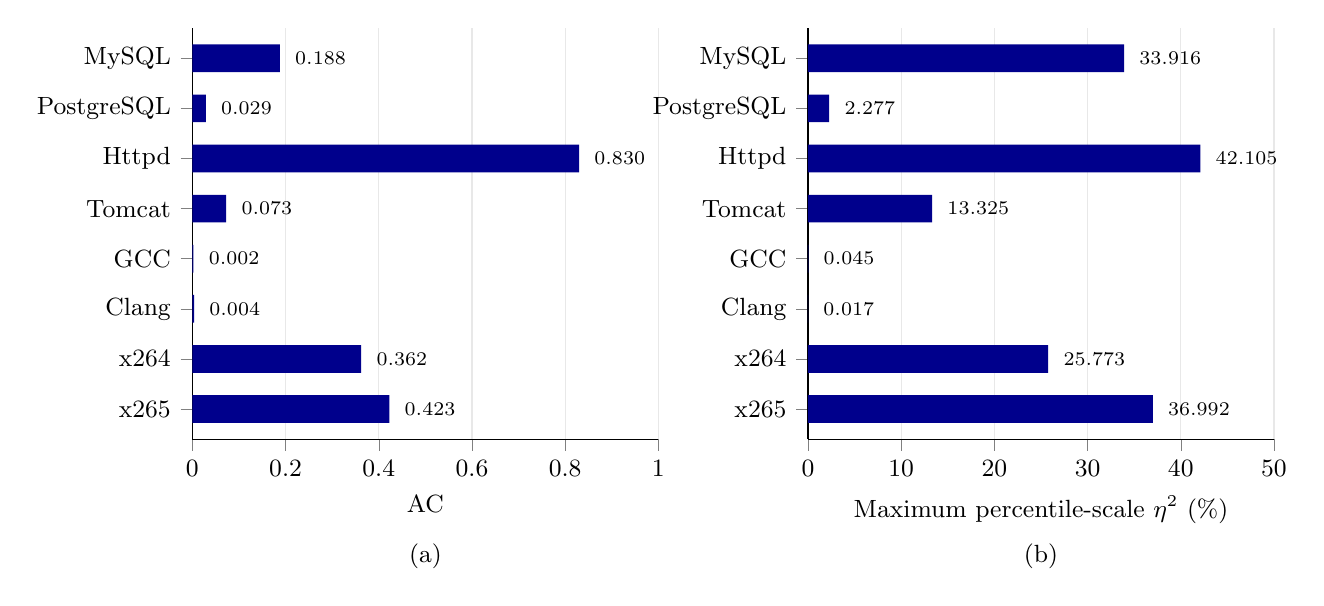
\begin{tikzpicture}
\begin{groupplot}[
  group style={group size=2 by 1, horizontal sep=1.9cm},
  width=7.5cm, height=6.8cm,
  xbar, /pgf/bar width=10pt,
  xmin=0, ymin=-0.6, ymax=7.6, y dir=reverse,
  ytick={0,1,2,3,4,5,6,7},
  yticklabels={MySQL,PostgreSQL,Httpd,Tomcat,GCC,Clang,x264,x265},
  tick label style={font=\small},
  label style={font=\small}, title style={font=\small},
  axis x line*=bottom, axis y line*=left,
  xmajorgrids=true, grid style={gray!18},
  tick align=outside, scaled x ticks=false,
  point meta=x, nodes near coords,
  nodes near coords align={horizontal},
  every node near coord/.append style={
    font=\scriptsize, text=black, anchor=west, xshift=2pt,
    /pgf/number format/.cd, fixed, fixed zerofill, precision=3
  },
  clip=false,
]
\nextgroupplot[
  xlabel={AC}, xmax=1.0,
  xtick={0,0.2,0.4,0.6,0.8,1.0},
]
\addplot[draw=none, fill=blue!55!black] coordinates {
(0.187789165918,0)
(0.028772796842,1)
(0.829791028437,2)
(0.072657411130,3)
(0.002325054443,4)
(0.003670631858,5)
(0.362267093907,6)
(0.422755012885,7)
};
\nextgroupplot[
  xlabel={Maximum percentile-scale $\eta^2$ (\%)},
  xmax=50, xtick={0,10,20,30,40,50},
]
\addplot[draw=none, fill=blue!55!black] coordinates {
(33.916169273577,0)
(2.277080291783,1)
(42.105128293698,2)
(13.325064875358,3)
(0.045202724507,4)
(0.016764055518,5)
(25.773324952866,6)
(36.992057317845,7)
};
\end{groupplot}
\node[anchor=north, font=\small]
  at ([yshift=-1.2cm]group c1r1.south) {(a)};
\node[anchor=north, font=\small]
  at ([yshift=-1.2cm]group c2r1.south) {(b)};
\end{tikzpicture}
\end{document}
